
\documentclass{beamer}


\mode<presentation>
{
  \usetheme{Hawke}
  \setbeamercovered{transparent}
}


\usepackage[english]{babel}
\usepackage[latin1]{inputenc}
\usepackage{times}
\usepackage[T1]{fontenc}
\usepackage{multimedia}


%%%%%%
% My Commands
%%%%%%

\newcommand{\ml}{{\sc matlab}}
\newcommand{\bb}{{\boldsymbol{b}}}
\newcommand{\bx}{{\boldsymbol{x}}}
\newcommand{\by}{{\boldsymbol{y}}}
\newcommand{\bfm}[1]{{\boldsymbol{#1}}}

%%%%

\title[Lecture 6] %
{Lecture 6 - Iterative Methods}


\author[I. Hawke]{I.~Hawke}

\institute[University of Southampton]%
{
  School of Mathematics, \\
  University of Southampton, UK
}

\date[Semester 1]{MATH3018/6141, Semester 1}

\subject{Numerical methods}

\pgfdeclareimage[height=0.5cm]{university-logo}{mathematics_7469}
\logo{\pgfuseimage{university-logo}}

\AtBeginSection[]
{
  \begin{frame}<beamer>
    \frametitle{Outline}
    \tableofcontents[currentsection]
  \end{frame}
}



\begin{document}

\begin{frame}
  \titlepage
\end{frame}

\section{Iterative Methods}

\subsection{Iterative Methods}

\begin{frame}
  \frametitle{Iterative Methods}

   We (still) want to solve the linear system
   \begin{equation*}
     A \bx = \bb.
   \end{equation*}
   Iterative methods build a \emph{sequence} of approximate
   solutions. Start from ``guess'' $\bx^{(0)}$ and compute
   approximations $\bx^{(1)}, \bx^{(2)}, \dots, \bx^{(N)}$ which
   converge to the exact solution. \pause

   \vspace{1ex}

   Standard ``notation'' is to split the matrix as
   \begin{equation*}
     A = N - P, \quad \implies \quad N \bx^{(i)} = P \bx^{(i - 1)} + \bb
   \end{equation*}
   and for Jacobi use $N=I$. \pause

   \vspace{1ex}

   Jacobi converges slowly: error drops by a constant amount each step.

\end{frame}

\subsection{Gauss-Seidel Method}

\begin{frame}
  \frametitle{Gauss-Seidel Method}

  In the Gauss-Seidel method split the coefficient matrix as
  \begin{equation*}
    A = I - (A_L + A_U)
  \end{equation*}
  as before. Choose
  \begin{align*}
    N & = I - A_L, \\
    P & = A_U.
  \end{align*}
  This makes the iteration scheme
  \begin{equation*}
    \bx^{(i)} =  A_L \bx^{(i)} + A_U \bx^{(i - 1)} + \bb, \quad i = 1,
    2, \dots
  \end{equation*} \pause

  Written in this form as $A_L$ \emph{strictly} lower
  triangular. Consider each component of the iteration scheme from the
  top down: each coefficient of $\bx^{(i)}$ is computed on the left
  before it is used on the right.

\end{frame}

\begin{frame}
  \frametitle{Example of Gauss-Seidel Method}

  As above we look at
  \begin{equation*}
    \begin{pmatrix}
      3 & 1 \\
      1 & 3
    \end{pmatrix}
    \begin{pmatrix}
      x_1 \\ x_2
    \end{pmatrix} =
    \begin{pmatrix}
      5 \\ 7
    \end{pmatrix} \rightarrow
    \begin{pmatrix}
      1 & \tfrac{1}{3} \\
      \tfrac{1}{3} & 1 \\
    \end{pmatrix}
    \begin{pmatrix}
      x_1 \\ x_2
    \end{pmatrix} =
    \begin{pmatrix}
      \tfrac{5}{3} \\ \tfrac{7}{3}
    \end{pmatrix}.
  \end{equation*}
  We have
  \begin{equation*}
    A_L =
    \begin{pmatrix}
      0 & 0 \\
      -1/3 & 0
    \end{pmatrix}, \quad
    A_U =
    \begin{pmatrix}
      0 & -1/3 \\
      0 & 0
    \end{pmatrix}
  \end{equation*}
  and hence the iteration algorithm becomes
  \begin{align*}
    \begin{pmatrix}
      x_1^{(i)} \\ x_2^{(i)}
    \end{pmatrix} & = \frac{1}{3} \left[
      \begin{pmatrix}
        -x_2^{(i-1)} \\ - x_1^{(i)}
      \end{pmatrix} +
      \begin{pmatrix}
        5 \\ 7
      \end{pmatrix} \right]
    = \frac{1}{3}
    \begin{pmatrix}
      5 - x_2^{(i-1)} \\ 7 - x_1^{(i)}
    \end{pmatrix}.
  \end{align*}
  If read row-by-row from the top we have always computed the
  $\bx^{(i)}$ entries before they are used.

\end{frame}


\begin{frame}
  \frametitle{Example of Gauss-Seidel Method 2}

  \begin{columns}
    \begin{column}{0.475\textwidth}
      The sequence has entries
      \begin{tabular}{|c|c c|}
        $i$ & $x_1$ & $x_2$ \\ \hline
        $0$ & $0$ & $0$ \\
        $1$ & $5 / 3$ & $16 / 9$ \\
        $2$ & $1.074074$ & $1.975309$ \\
        $5$ & $1.000102$ & $1.999966$ \\
        $10$ & $1.000000$ & $2.000000$ \\
        $100$ & $1.000000$ & $2.000000$
      \end{tabular}
    \end{column}
    \begin{column}{0.525\textwidth}
      \begin{center}
        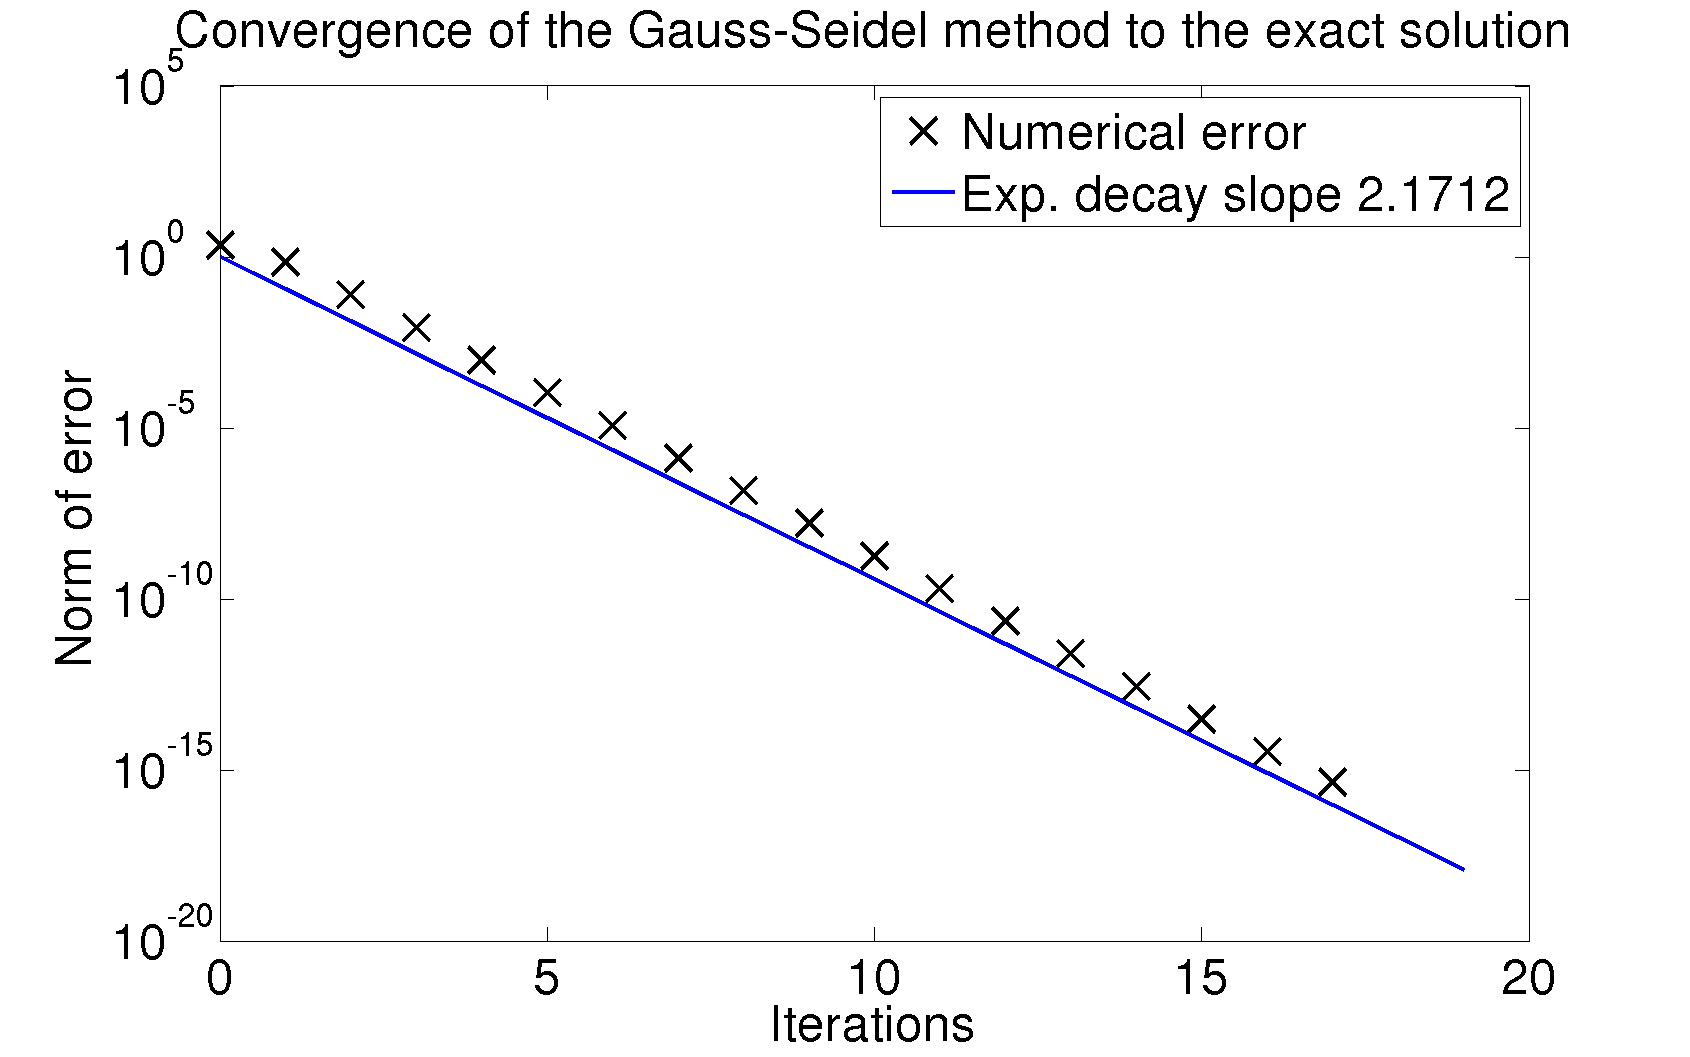
\includegraphics[width=\textwidth]{figures/GaussSeidel1}
      \end{center}
    \end{column}
  \end{columns}

  \vspace{1ex}

  A starting ``guess'' of $\bx = \bfm{0}$ appears to converge to $\bx
  = (1, 2)^T$. The convergence is exponential with a slope $\sim 2$,
  much faster than Jacobi's Method.

\end{frame}


\subsection{Successive Over Relaxation}

\begin{frame}
  \frametitle{Successive Over Relaxation}

  View the sequence as repeated ``corrections'' to the previous term,
  \begin{equation*}
    \bx^{(i)} = \bx^{(i-1)} + \bfm{c},
  \end{equation*}
  where correction is based e.g.\ on Gauss-Seidel method,
  \begin{equation*}
    \bfm{c} = A_L \bx^{(i)} + (A_U - I) \bx^{(i-1)} + \bb.
  \end{equation*} \pause

  Modify correction by factor $\omega$:
  \begin{equation*}
    \bx^{(i)} = \bx^{(i-1)} + \omega \bfm{c}.
  \end{equation*} \pause

  \emph{A priori} best value of $\omega$ not clear.  Typically it is
  set close to one. However, poor choices may cause the algorithm to
  diverge!

\end{frame}


\begin{frame}
  \frametitle{Example of SOR Method 1}

  \begin{columns}
    \begin{column}{0.475\textwidth}
      Solving the previous example using $\omega = 1.035$, the
      sequence has entries
      \begin{tabular}{|c|c c|}
        $i$ & $x_1$ & $x_2$ \\ \hline
        $0$ & $0$ & $0$ \\
        $1$ & $1.725000$ & $1.819875$ \\
        $2$ & $1.036768$ & $1.993619$ \\
        $5$ & $0.999999$ & $2.000000$ \\
        $10$ & $1.000000$ & $2.000000$ \\
        $100$ & $1.000000$ & $2.000000$
      \end{tabular}
    \end{column}
    \begin{column}{0.525\textwidth}
      \begin{center}
        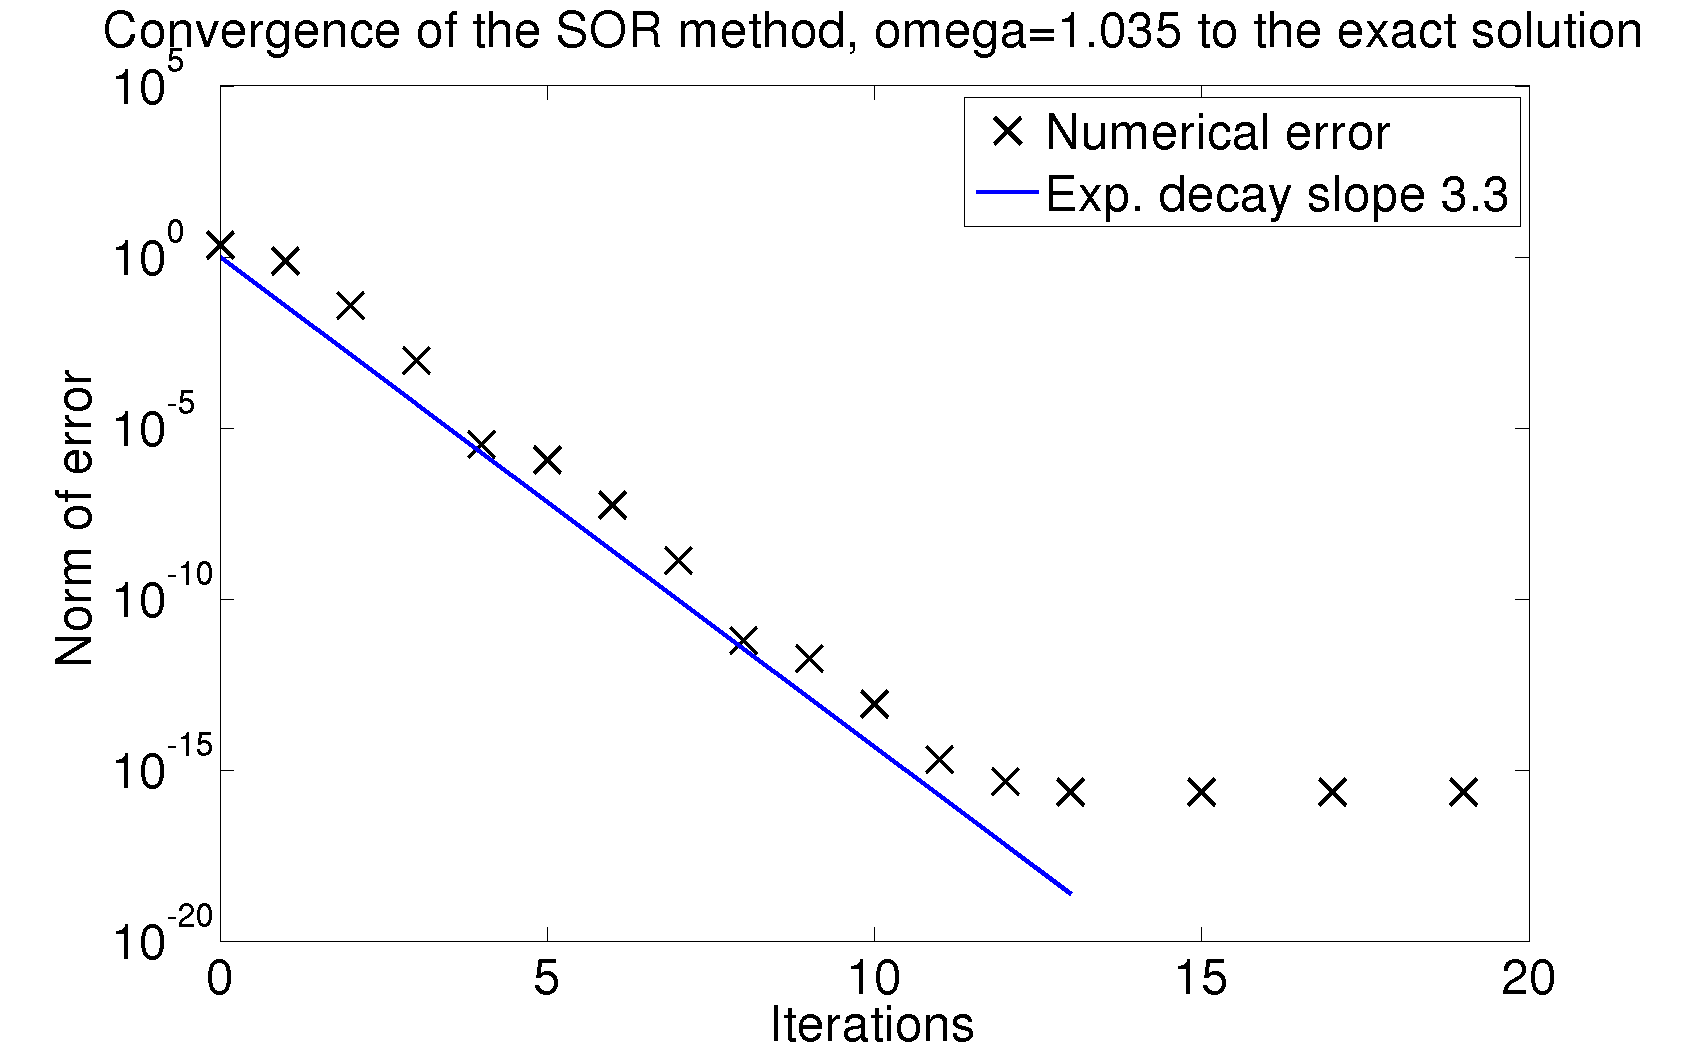
\includegraphics[width=\textwidth]{figures/SOR1}
      \end{center}
    \end{column}
  \end{columns}

  \vspace{1ex}

  A starting ``guess'' of $\bx = \bfm{0}$ appears to converge to $\bx
  = (1, 2)^T$. The convergence is exponential with a slope $\sim 3$,
  the fastest method so far.

\end{frame}

\begin{frame}
  \frametitle{Example of SOR Method 2}

  \begin{columns}
    \begin{column}{0.475\textwidth}
      Solving the previous example using $\omega = 1.2$, the
      sequence has entries
      \begin{tabular}{|c|c c|}
        $i$ & $x_1$ & $x_2$ \\ \hline
        $0$ & $0$ & $0$ \\
        $1$ & $2.000000$ & $2.000000$ \\
        $2$ & $0.800000$ & $2.080000$ \\
        $5$ & $0.998221$ & $2.000430$ \\
        $10$ & $1.000000$ & $2.000000$ \\
        $100$ & $1.000000$ & $2.000000$
      \end{tabular}
    \end{column}
    \begin{column}{0.525\textwidth}
      \begin{center}
        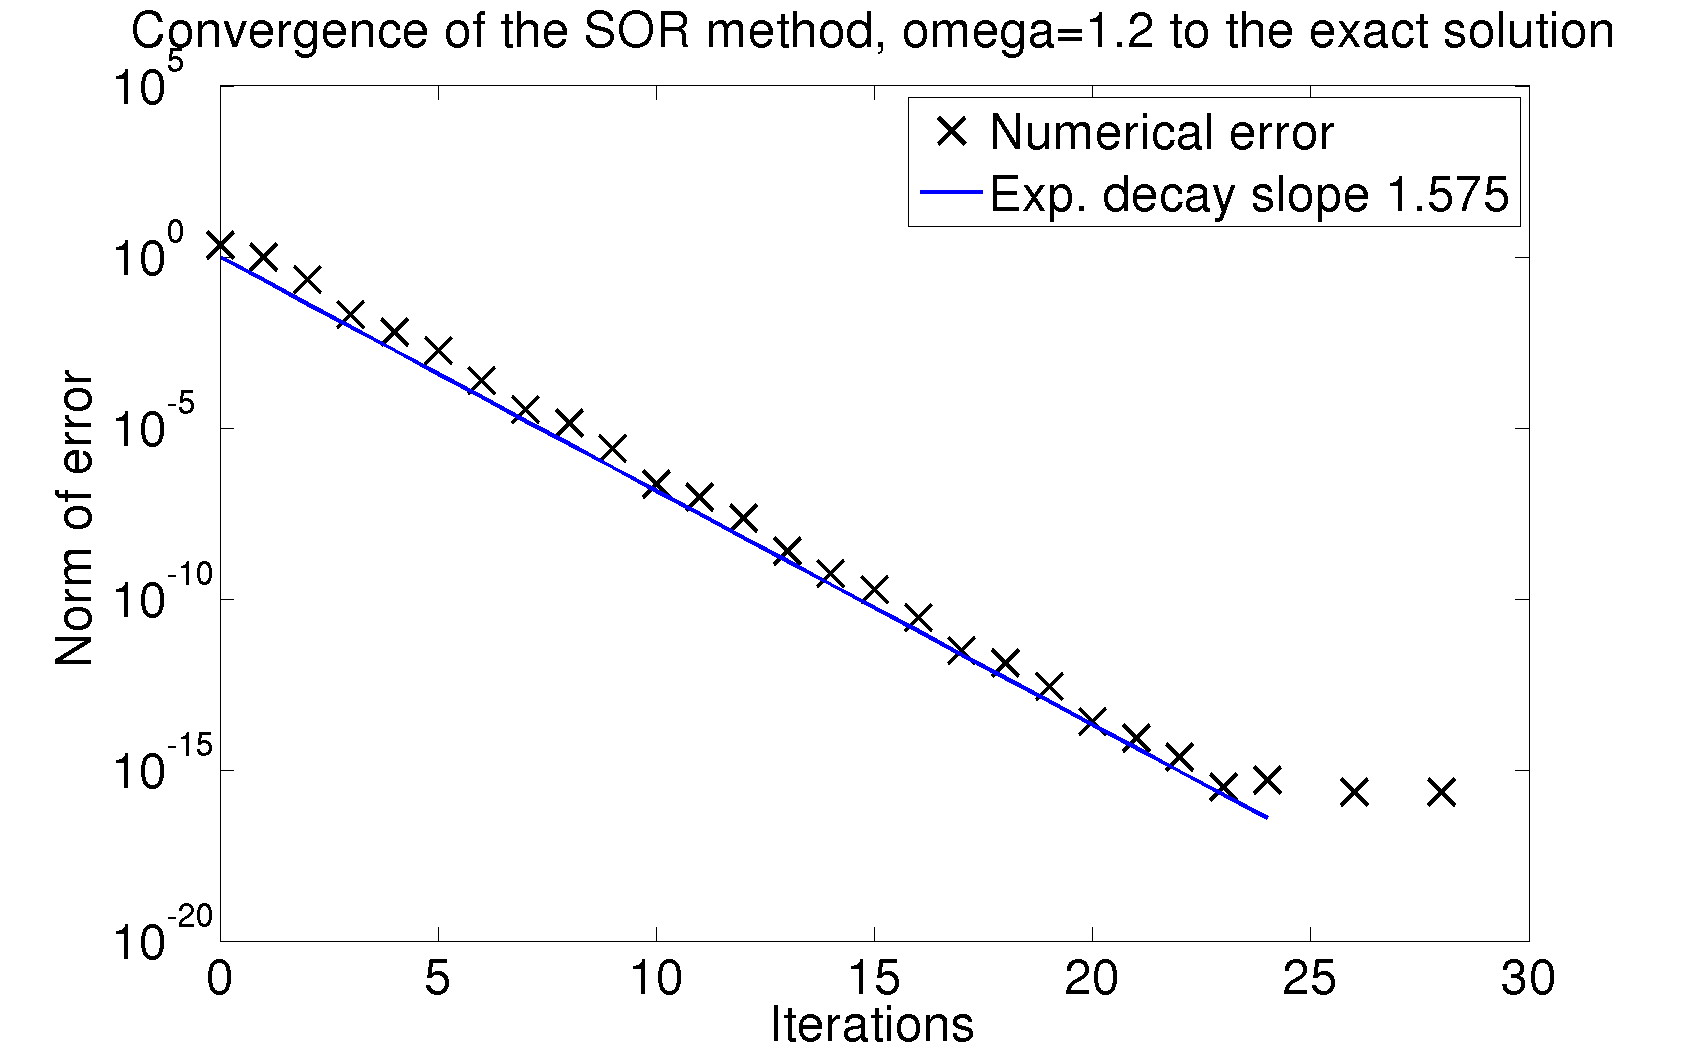
\includegraphics[width=\textwidth]{figures/SOR2}
      \end{center}
    \end{column}
  \end{columns}

  \vspace{1ex}

  A starting ``guess'' of $\bx = \bfm{0}$ appears to converge to $\bx
  = (1, 2)^T$. The convergence is exponential with a slope $\sim 1.6$,
  which is not as good as Gauss-Seidel.

\end{frame}

\begin{frame}
  \frametitle{The relaxation parameter}

  \begin{center}
    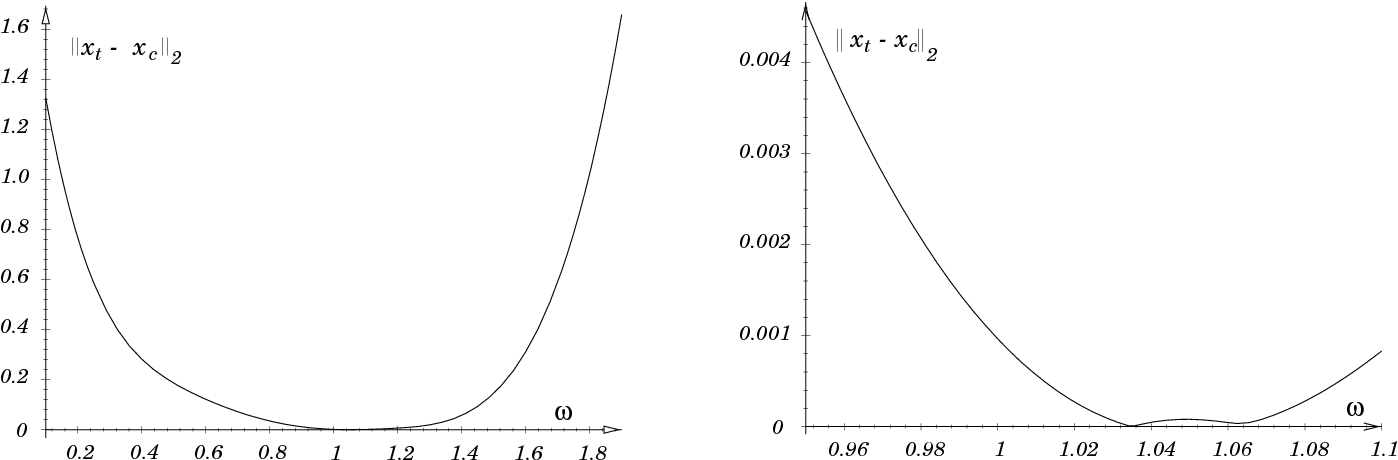
\includegraphics[width=0.9\textwidth]{figures/SOR}
  \end{center}
  The norm of the error obtained with SOR after four iterations.  The
  convergence behaviour depends in a highly non-trivial way on
  $\omega$.

  \vspace{1ex}

  SOR algorithms are much harder to analyze than Jacobi or
  Gauss-Seidel.

\end{frame}


\subsection{Convergence Analysis}

\begin{frame}
  \frametitle{Convergence analysis}

  Two theorems about \emph{when} these methods will work:

  \vspace{2ex}

  {\bf Theorem 1}: If the coefficient matrix $A$ is \emph{strictly}
  diagonally dominant then both the Jacobi method and the Gauss-Seidel
  method will converge.

  \vspace{2ex}

  {\bf Theorem 2}: If the coefficient matrix $A$ is symmetric and
  positive definite then the Gauss-Seidel method will converge.

\end{frame}


\section{Other matrix operations}


\subsection{Other matrix operations}

\begin{frame}
  \frametitle{Other matrix operations}

  We have so far only considered the linear system
  \begin{equation*}
    A \bx = \bb.
  \end{equation*}
  We have given methods to solve this system accurately without
  computing the matrix inverse or determinant. However, these methods
  can also be used to efficiently and accurately compute these
  quantities.
\end{frame}

\begin{frame}
  \frametitle{Determinants}

  Given the $LU$ decomposition we have
  \begin{equation*}
    \det (A) = \det(L) \times \det(U), \quad \text{and} \quad \det(U)
    = \prod_{i=1}^n u_{ii}.
  \end{equation*}
  Choose $\ell_{ii}=1$ giving $\det(L) = 1$: determinant
  follows. \pause

  \vspace{1ex}

  Similarly Gaussian elimination with partial pivoting gives
  \begin{equation*}
    \det(A) = \pm \prod_{i=1}^n u_{ii},
  \end{equation*}
  where the sign depends on the number of row swaps performed.\pause

  \vspace{1ex}

  {\bf Note:} Gaussian elimination, and hence finding the determinant,
  is an ${\cal O}(n^3)$ operation.  The expansion in minors is an
  ${\cal O}(n!)$ operation.

\end{frame}

\begin{frame}
  \frametitle{Matrix inversion}

  Solving for the matrix inverse can be written as a set of linear
  system problems. We write
  \begin{equation*}
    A A^{-1} = I
  \end{equation*}
  and consider each column of $A^{-1}$ as a separate problem. \pause
  Writing $\bfm{c}_i$ for the (unknown) column of $A^{-1}$ we have
  \begin{equation*}
    A \bfm{c}_i =
    \begin{pmatrix}
       \vdots \\ 0 \\ 1 \\ 0 \\ \vdots
    \end{pmatrix}
  \end{equation*}
  where the $1$ appears in the $i^{\text{th}}$ row. \pause

  \vspace{1ex}

  This finds the inverse by solving $n$ linear systems, which is much
  faster than evaluating the $n+1$ determinants required by Cramer's
  rule.

\end{frame}

\section{Summary}

\subsection{Summary}

\begin{frame}
  \frametitle{Summary}

  \begin{itemize}
  \item Iterative methods are often based on the split
    \begin{equation*}
      A = N - P.
    \end{equation*}
  \item Convergence depends on $M = N^{-1}P$.
  \item Jacobi chooses $N = I$ and converges slowly.
  \item Gauss-Seidel chooses $N = I - A_U$ and uses coefficients as
    soon as they become available. Slightly harder to code, it
    converges faster than Jacobi.
  \item SOR tries to ``accelerate'' the convergence of Gauss-Seidel
    depending on a parameter $\omega$. It can be faster, but the
    behaviour depends non-trivially on $\omega$ and it is very
    difficult to analyze.
  \item Strict diagonal dominance is sufficient for convergence of
    both Jacobi and Gauss-Seidel methods.
  \item Computing determinants and inverses from the solution of
    linear systems is usually much faster than ``standard''
    techniques.
  \end{itemize}

\end{frame}

\end{document}



%%% Local Variables:
%%% mode: latex
%%% TeX-master: t
%%% End:
